\documentclass[border=10pt]{standalone} 
\usepackage{verbatim}
\usepackage{tikz}
\usetikzlibrary{arrows,decorations.markings}
\begin{document}
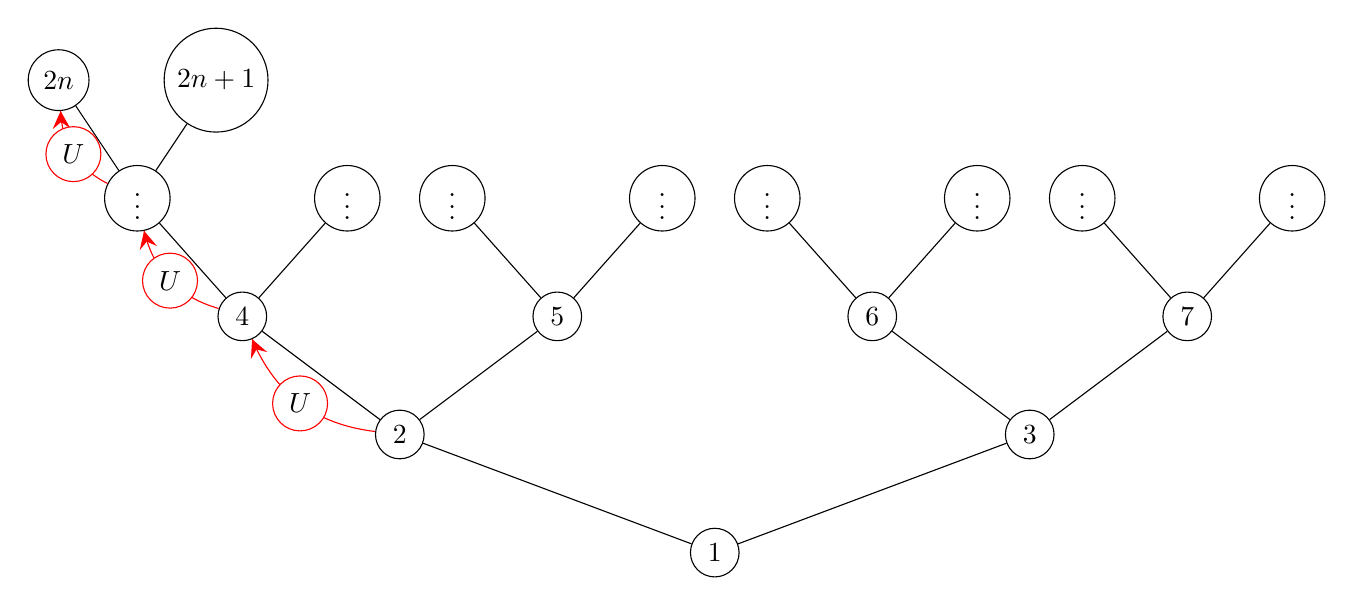
\begin{tikzpicture}[
  grow=up,
  every node/.style = {shape=circle, draw, align=center,minimum size = 1 pt},
  level/.style={sibling distance=80mm/#1}
  ]
  \node (1) {1}
    child
    {
        node (3) {3}
        {
          child
          {
              node (7) {7}
              child {node {$\vdots$}}
              child {node {$\vdots$}}
          }
          child
          {
              node (6) {6}
              child {node {$\vdots$}}
              child {node {$\vdots$}}
          }
        }
    }
    child
    {
        node (2) {2}
        {
          child
          {
              node (5) {5}
              child {node (11) {$\vdots$}}
              child {node (10) {$\vdots$}}
          }
          child
          {
              node (4) {4}
              child {node (9) {$\vdots$}}
              child
              {
                node (8) {$\vdots$}
                child {node (17) {$2n+1$}}
                child {node (16) {$2n$}}
              }
          }
        }
    };

  \tikzset{EdgeUp/.style   = {red, bend left,decoration={markings,mark=at position 1 with
    {\arrow[scale=2,>=stealth]{>}}},postaction={decorate}}}
  \tikzset{LabelStyle/.style =   {draw, fill=white, text=black,minimum size = 1 pt}}

  \draw[EdgeUp](2) to node[LabelStyle]{$U$} (4);
  \draw[EdgeUp](4) to node[LabelStyle]{$U$} (8);
  \draw[EdgeUp](8) to node[LabelStyle]{$U$} (16);

\end{tikzpicture}


\end{document}
